\subsection{进一步近似}
更令人感兴趣的是鞍点方程(5.3)的非均匀解。通常需要数值分析的方法来得到这种平均场解的精确描述。数值方法的讨论推迟到第5.3节;在这里,我们考虑进一步的分析近似,使不均匀的鞍点方程易于处理。这些近似基于第3.4节中提出的方案,用于估计外部势场中单链的统计特性。
\subsubsection{弱不均匀性-RPA}
可以与平均场近似一起应用的一种重要的近似类型是弱不均匀性扩展。在方程(5.3)的解几乎是一致的情况下,我们可以用方程(3.113)类比得出
\begin{equation}
w^*(\br)=w_0+\omega^*(\br)
\end{equation}
其中$w_0\equiv(1/V)\int w^*(\br)\mathrm{d}\br$是体积平均的平均场势场,假设偏差$\omega^*(\br)$与$w_0$相比在任何地方都很小,可以遵循3.4.1节的流程来产生弱的不均匀性扩展。这种扩展在聚合物文献中通常称为随机相近似,或RPA(de Gennes,1969;de Gennes,1979)。我们用规范模型A来说明它。

规范模型A的鞍点方程在方程(5.11)中给出。代替方程(5.18)并应用方程(3.134)和(4.75)导出以下扩展:
\begin{equation}
u_0^{-1}\omega^*(\br)+\rho_0N\int g_D(\left|\br-\br'\right|)\omega^*(\br')\mathrm{d}\br'+O((\omega^*)^2)=0
\end{equation}
其中方程(5.12)用于取消主导齐次项,$g_D$是方程(3.133)的Debye函数。方程(5.19)的唯一解是$\omega^*(\br)=0$,这与我们之前的声明一致,即规范模型A的整体或具有周期性边界条件的单元的唯一鞍点是均匀解$w^*(\br)=w_0$。

RPA扩展还可用来观察密度函数$F[\rho]$的形式,这是第4.10节DFT形式的核心,在平均场近似中,规范模型A的方程(4.207)简化为
\begin{equation}
\rho(\br)\approx\tilde{\rho}(\br;[iw^*+J])
\end{equation}
我们用$\rho(\br)$的简写代替$\left\langle\hat{\rho}(\br)\right\rangle_J$。该等式确定由任意外部势场$J(\br)$产生的平均段密度$\rho(\br)$。此外,在平均场近似中,方程(4.205)的配分函数简化为$\calZ_C[J]\approx\calZ_0\exp(-H[w^*,J])$,在这两个表达式中,鞍点$w^*(\br)$由下式确定
\begin{equation}
\frac{\delta H[w,J]}{\delta w(\br)}\bigg|_{w=w^*}=u_0^{-1}w^*(\br)+i\tilde{\rho}(\br;[iw^*+J])=0
\end{equation}
通过选择$J$,使其幅值较弱并且具有较好的体积平均值,即$(1/V)\int J(\br)\mathrm{d}\br=0$,方程(5.21)的右端可以类似于方程(5.19)的RPA扩展得出。在$J$的领先秩序,
\begin{equation}
\begin{aligned}
\int[u_0^{-1}\delta(\br-\br')&+\rho_0Ng_D(\left|\br-\br'\right|)]\omega^*(\br')\mathrm{d}\br'\\
&=i\rho_0N\int g_D(\left|\br-\br'\right|)J(\br')+O(J^2)
\end{aligned}
\end{equation}
该结果的傅里叶变换产生以下关于$\omega^*$和$J$的公式:
\begin{equation}
\hat{\omega}^*(\bk)=\frac{iu_0\rho_0N\hat{g}_D(x)}{1+u_0\rho_0N\hat{g}_D(x)}\hat{J}(\bk)+O(J^2)
\end{equation}
其中$x=k^2R_g^2$是无量纲的平方波数,其具有未受扰动的回旋半径的平方,$R_g^2=Nb^2/6$。

下一步是使用方程(5.23)和(3.131)扩展方程(4.206)中给出的函数$H[w^*,J]$。这将得出:
\begin{equation}
H[w^*,J]=H_0-\frac{1}{2V}\sum\limits_{\bk}\frac{\rho_0N\hat{g}_D(x)}{1+u_0\rho_0N\hat{g}_D(x)}\hat{J}(\bk)\hat{J}(-\bk)+O(J^3)
\end{equation}
其中$H_0\equiv(1/2u_0)Vw_0^2+w_0Nn$是对哈密顿量的均匀贡献。构造自由能函数$F[\rho]$所需的最后一步是通过方程(4.199)利用勒让德变换将$J$变为$\rho$,即
\begin{equation}
F[\rho]=-\ln\calZ_0+H[w^*,J]-\int J(\br)\rho(\br)\mathrm{d}\br
\end{equation}
这个变换需要扩展方程(5.20)来建立$J$和$\rho$之间的关系。应用方程(3.134)得
\begin{equation}
\widehat{\Delta\rho}(\bk)=-\frac{\rho_0N\hat{g}_D(x)}{1+u_0\rho_0N\hat{g}_D(x)}\hat{J}(\bk)+O(J^2)
\end{equation}
其中$\Delta\rho(\br)\equiv\rho(\br)-\rho_0$是单体密度场的不均匀部分。结合方程(5.24)-(5.26)得到所需的自由能泛函
\begin{equation}
F[\rho]=F_0+\frac{1}{2V}\sum\limits_{\bk}\left(\frac{1}{\rho_0N\hat{g}_D(x)}+u_0\right)\widehat{\Delta\rho}(\bk)\widehat{\Delta\rho}(-\bk)+O(\Delta\rho^3)
\end{equation}
其中$F_0$是均匀流体的平均场自由能。

方程(5.27)是对应于模型A的弱非均匀聚合物溶液的自由能(以$k_BT$为单位)的表达式。在适用平均场近似且密度不均匀性小的程度上是有效的。正如将在第6章讨论的那样,平均场近似适用于模型A,其浓度足够高满足
\begin{equation}
C\gg B\equiv\frac{u_0N^2}{R_g^3}
\end{equation}
其中$C=nR_g^3/V$是在方程(5.5)中引入的无量纲链浓度,$B$是无量纲消除体积参数。

方程(5.27)的一个有用的应用是估计聚合物溶液的均相相对于小幅度密度扰动的稳定性。通过检查二次系数可以确定稳定性。
\begin{equation}
\hat{\Gamma}_2(k)=\frac{1}{\rho_0N\hat{g}_D(k^2R_g^2)}+u_0
\end{equation}
作为波数$k=\left|\bk\right|$的函数。由于$\hat{g}_D(x)$是$x$的单调递减函数,因此,$\hat{\Gamma}_2(k)$的最小值与$k=0$一致。均匀相或螺旋线的稳定极限因此对应于
\begin{equation}
\hat{\Gamma}_2(0)=\frac{1}{\rho_0N}+u_0=0
\end{equation}
由此得出,在平均场近似中,当$u_0$达到负值$-1/(\rho_0N)$时,模型A呈现出长波长(k=0)不稳定性,这种不稳定性产生宏观相分离成两个液晶相:一种富含聚合物;另一种富含溶剂。尽管模型A对于消除体积参数$u_0$的负值定义不正确,但是对应于较差的溶剂条件,平均场螺旋线通过方程(5.30)正确定位。然而,为了研究在穿过螺旋线边界时出现的新相的出现和性质,我们有必要改用模型B。

RPA扩展可用于研究第4章中描述的许多其他模型的均相稳定性。通常,人们获得类似于方程(5.27)的表达式,即
\begin{equation}
F[\rho]=F_0+\frac{1}{2V}\sum\limits_{\bk}\hat{\Gamma}_2(k)\widehat{\Delta\rho}(\bk)\widehat{\Delta\rho}(-\bk)+O(\Delta\rho^3)
\end{equation}
但是$\hat{\Gamma}_2(k)$的形式取决于模型。对于模型B,可以得到
\begin{equation}
\hat{\Gamma}_2(k)=v_0\left(\frac{1}{\phi_{P0}N\hat{g}_D(k^2R_g^2)}+\frac{1}{\phi_{S0}}-2\chi_{PS}\right)
\end{equation}
其中$\phi_{P0}\equiv n_PNv_0/V$是平均聚合物体积分数,$\phi_{S0}=n_Sv_0/V=1-\phi_{P0}$是平均溶剂体积分数,$v_0$是每个聚合物链段的体积和溶剂分子。在模型B中,$\Delta\rho(\br)$可以解释为$\Delta\rho_P(\br)$或$\Delta\rho_S(\br)$,因为它是由于其不可压缩性而导致的,即$\Delta\rho_P(\br)=-\Delta\rho_S(\br)$。对于较小聚合物体积分数,$\phi_{P0}\gg 1$,当我们使$u_0=v_0(1-2\chi_{PS})$对应时,可得到与方程(5.30)相对应的稳定阈值。然而,对于模型B,可以通过假定$\hat{\Gamma}_2(0)=0$获得的液-液相分离的螺旋线边界不同于在更高聚合物浓度下的模型A的螺旋线。实际上,模型B的表达式与熟悉的聚合物溶液的Flory-Huggins晶格理论的螺旋线一致(de Gennes,1979)。

最后一个例子对应于不可压缩的AB两嵌段共聚物熔体。在一篇经典论文(Leibler,1980)中,Leibler计算出模型E的RPA扩展到密度不均匀性的四阶,$\Delta\rho\equiv\Delta\rho_A=-\Delta\rho_B$。对于相等的统计分段长度,$b\equiv b_A=b_B$,扩展中的二次系数具有以下形式
\begin{equation}
\hat{\Gamma}_2(k)=\frac{v_0}{N}\left[\gamma(k^2R_g^2,f)-2\chi_{AB}N\right]
\end{equation}
其中$R_g^2=Nb^2/6$是共聚物的无扰动回旋半径,函数$\gamma(x,f)$由下式定义
\begin{equation}
\gamma(x,f)=\frac{\hat{g}(1,x)}{\hat{g}(f,x)\hat{g}(1-f,x)-(1/4)[\hat{g}(1,x)-\hat{g}(f,x)-\hat{g}(1-f,x)]^2}
\end{equation}
在这个表达式中,$\hat{g}(f,x)$是修正后的Debye函数
\begin{equation}
\hat{g}(f,x)\equiv\frac{2}{x^2}[fx+\exp(-fx)-1]
\end{equation}
在固定嵌段共聚物组成$f$(A嵌段的体积分数)下,函数$\gamma(x,f)$在$x$,$x_m(f)$的非零值处具有$f$依赖的最小值,由下式给出:
\begin{equation}
\frac{\partial\gamma(x,f)}{\partial x}\bigg|_{x=x_m}=0
\end{equation}
在对称两嵌段共聚物的情况下,$f=1/2$,$x_m(1/2)=3.785$,因此,均相嵌段共聚物熔体中最不稳定的密度模式$\widehat{\Delta\rho_A}(\bk)$具有非零波数$k=[x_m(f)]^{1/2}/R_g$,对应于$\lambda=2\pi R_g/[x_m(f)]^{1/2}$。这种有限长度尺度不稳定性表示波长接近$\lambda$的周期性中间相的开始。

从$\gamma(x_m,f)-2\chi_{AB}N=0$的关系中得到了共聚物熔体均相分离的稳定极限。这在$\chi_{AB}N$对$f$的平面上产生一条曲线,该曲线显示在平均场近似下,均相熔体是稳定的或不稳定的。在$f=1/2$时,我们观察到对称共聚物熔体的稳定极限为$\chi_{AB}N=10.495$。在平均场理论中,在$f=1/2$以外的所有部分中,相与各种有序之间的有序-无序跃迁是一种一级相变,因此需要更高的展开项来精确地区分这两种变化曲线。同时也决定了在通过这个过程时所出现的有序性的对称性(Leibler,1980)。在实践中,这种高阶分析变得非常简单,并且仅限于弱有序的再结晶技术-所谓的弱偏析技术已经发展到了这样一个阶段,即对全平均场方程的直接数值方法,这是5.3节的主题,一般用于研究嵌段共聚物和溶液中的生成。

理解聚合物溶液和嵌段共聚物对应的线性特征的物理根源是非常重要的。一种聚合物溶液,因为存在与组织链相关联的熵罚因子,以支持非均匀段密度剖面。由此可以看出,这种自由能罚因子随$k$的增大而增加,对于$k\gg R_g^{-1}$,则以$k^2$的形式生长。同样的方法也适用于嵌段共聚物,从大$k$的行为可以推断出。然而,嵌段共聚物熔体不能承受任意长波长(小$k$)成分的波动,因为这将需要拉伸单个共聚物链,使$A$段和$B$段在很长的距离内分离。这种拉伸导致了一种熵损失,其根据方程(5.33)增长为$k^2$当$k\rightarrow 0$。因此,连接每个共聚物的两个嵌段的化学键的集体表现是优选的波数,$k_m=\sqrt{x_m}/R_g$,存在共聚物熔体中的组成波动。
该优选的波数反应了对共聚物分子量和平均组成敏感的构象熵损失,更一般地,对嵌段共聚物结构敏感,尽管由$k_m$设定的长度尺寸与在ODT处形成的周期性中间相的晶格常数相关,但是在进入相图的有序区域时,晶格常数以RPA分析无法预测的方式发展(Almdal,1990;Matsen和Bates,1996b)
\begin{figure}[H]
      \centering
      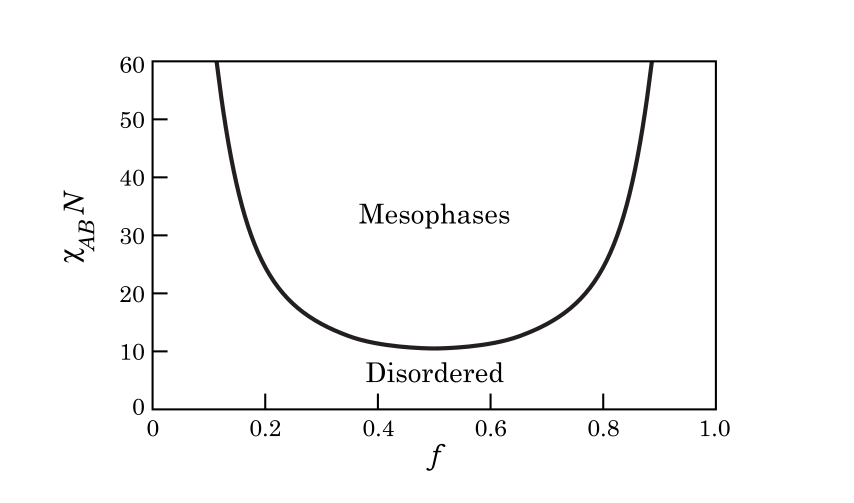
\includegraphics[width=12cm]{./figures/4.png}
      \caption{不可压缩AB两嵌段共聚物熔体的Spinodal曲线由模型E描述的区域。表示为“无序”的区域表示块偏析强度$\chi_{AB}N$和组成$f$的值,其中均匀的,组成无序的相对于小幅度组成扰动是稳定的。表示为“Mesophases”的区域对应于$\chi_{AB}N$和$f$,使得无序相相对于小振幅,有限波长组成扰动不稳定,表明微相分离的开始。在平均场近似中,一阶ODT曲线在接近所示的螺旋线的任何地方都是,并且两条曲线在$f=1/2$,$\chi_{AB}N=10.495$处合并,其中转变被预测为二阶的。}
\end{figure}

RPA扩展中的二次系数$\hat{\Gamma}_2(k)$与由下式定义的均匀流体相的结构因子$S(k)$相关联。
\begin{equation}
S(k)=V^{-1}\int\mathrm{d}\br\int e^{-i\bk\cdot(\br-\br')}\left\langle[\hat{\rho}(\br)-\rho_0][\hat{\rho}(\br')-\rho_0]\right\rangle_0\mathrm{d}\br'
\end{equation}
其中下标$0$平均表示相互作用系统中的无场,$J=0$,整体平均上链构象。结构因子与用中子,X射线或光进行的辐射散射实验有关(Hansen和McDonald,1986)。$\Gamma_2(k)$和$S(k)$之间的形式联系是通过应用线性理论建立的,对于模型A来说意味着
\begin{equation}
\left\langle\hat{\rho}(\br)\right\rangle_J=\rho_0-\int\left\langle\hat{\rho}(\br)\hat{\rho}(\br')\right\rangle_0J(\br')\mathrm{d}\br'+O(J^2)
\end{equation}
该公式是通过$J$中的直接扰动扩展得出的,假设$\int J(\br)\mathrm{d}\br=0$,表明静态相应的线性函数与无场的密度-密度相关函数成比例,即
\begin{equation}
\frac{\delta\left\langle\hat{\rho}(\br)\right\rangle_J}{\delta J(\br')}\bigg|_{J=0}=-\left\langle\hat{\rho}(\br)\hat{\rho}(\br')\right\rangle_0
\end{equation}
如果我们从密度泛函理论的讨论中引用(4.200),那么得到
\begin{equation}
\frac{\delta^2F[\left\langle\hat{\rho}\right\rangle_J]}{\delta\left\langle\hat{\rho}(\br)\right\rangle_J\delta\left\langle\hat{\rho}(\br')\right\rangle_J}=-\frac{\delta J(\br)}{\delta\left\langle\hat{\rho}(\br')\right\rangle_J}
\end{equation}
结合方程(5.39)和(5.40)得出
\begin{equation}
\frac{\delta^2F[\rho]}{\delta\rho(\br)\delta\rho(\br')}\bigg|_{J=0}=[\left\langle\hat{\rho}(\br)\hat{\rho}(\br')\right\rangle_0]^{-1}
\end{equation}
我们已经恢复了本节的简化符号$\rho\equiv\left\langle\hat{\rho}\right\rangle_J$,右端的上标$-1$表示方程(C.29)意义上的函数逆。最后,在傅里叶空间,
\begin{equation}
\frac{\partial^2F[\rho]}{\partial\widehat{\Delta\rho}(\bk)\partial\widehat{\Delta\rho}(-\bk)}\bigg|_{\Delta\rho=0}=\frac{\hat{\Gamma}_2(k)}{V}=\frac{1}{VS(k)}
\end{equation}
它建立了所需的关联$S(k)=1/\hat{\Gamma}_2(k)$。这是无序相波动的一般结果,尽管RPA公式(5.29),(5.32)和(5.33)依赖于平均场近似。这些表达式在散射实验中都得到了很好的测试(des Cloizeaux和Jannink,1990;Bates和Hartney,1985)。
最后,我们指出平均场近似中出现的不一致性。直接应用方程(4.78)与平均场表达式$\left\langle w(\br)w(\br')\right\rangle\approx w^*(\br)w^*(\br')$导出$S(k)=u_0^{-1}$的无序相位模型A,当忽略$w$场波动时无序相无结构的这种明显结果与严格的平均场近似一致。相反,当与方程(5.29)结合时,上面得到的公式$S(k)=1/\hat{\Gamma}_2(k)$对模型A的无序相中的密度波动做出了非常不同的陈述,这种不一致是众所周知的在相互作用场理论的平均场近似中(Amit,1984;Goldenfeld,1992)。在精确计算中,这两种方法当然必须提供相同的结果,然而,在精确波动公式$S(k)=1/\hat{\Gamma}_2(k)$中使用$\hat{\Gamma}_2(k)$的RPA表达式实际上提供了超出严格的平均场理论并且在高斯水平中包含$w$场波动的结果。这一点将在第6章进一步讨论。
\subsubsection{慢梯度}
可以与平均场近似相结合的另一种有用的近似方案是3.4.2节的慢梯度扩展。这里的基本假设是自洽场$w^*(\br)$和相关的分段密度$\left\langle\hat{\rho}(\br)\right\rangle$在长度尺寸上缓慢变化,与聚合物回旋半径$R_g$相当。同样,我们用模型A说明了这一点,并着重于密度函数$F[\rho]$的构造。如Tang和Freed(1991)所示,大型规范集合证明了开发这种梯度扩展最方便。

起点是平均场表达式(5.20)的类似大型规范版本,即
\begin{equation}
\rho(\br)=\tilde{\rho}_G(\br;[\mu^*])
\end{equation}
我们定义了$\mu^*(\br)\equiv iw^*(r)+J(\br)$并再次使用简写$\rho(\br)$代替$\left\langle\hat{\rho}(\br)\right\rangle$。将此结果与方程(3.157)和(4.76)相结合得到
\begin{equation}
\rho(\br)=zNe^{-N\mu^*(\br)}\left\{1+R_g^2\left(\frac{N^2}{6}\left|\nabla\mu^*\right|^2-\frac{N}{3}\nabla^2\mu^*\right)+\cdots\right\}
\end{equation}
其中被忽略的项是$\mu^*$的梯度的四阶和更高项。方程(5.44)将$\rho$表示为$\mu^*$的梯度展开。可以反解该函数关系以在$\rho$的梯度中表示$\mu^*$,即
\begin{equation}
\begin{aligned}
\mu^*(\br)=&-\frac{1}{N}\ln[\rho(\br)/zN]\\
&-\frac{R_g^2}{6N[\rho(\br)]^2}\left|\nabla\rho\right|^2+\frac{R_g^2}{3N\rho(r)}\nabla^2\rho+\cdots
\end{aligned}
\end{equation}
大规范集合中模型A的平均场方程意味着$iw^*(\br)=\u_0\rho(\br)$。因此,通过从等式(5.45)的两端减去$u_0\rho$来获得$\rho$的梯度中的$J=\mu^*-iw^*=\mu^*-u_0\rho$的扩展。

下一步是研究大规模哈密顿量的扩展
\begin{equation}
H_G[w^*,J]=\frac{1}{2u_0}\int[w^*(\br)]^2-zVQ[\mu^*]\mathrm{d}\br
\end{equation}
在$J$的梯度也即在$\rho$的梯度。使用方程(3.156)和方程(5.45)得到
\begin{equation}
H_G[w^*,J]=-\int\left(\frac{1}{N}\rho+\frac{u_0}{2}\rho^2-\frac{R_g^2}{3N}\nabla^2\rho+\cdots\right)\mathrm{d}\br
\end{equation}
最后,为了完成计算,我们通过以下方式通过Legendre变换把$J$的函数变换到$\rho$的函数
\begin{equation}
F[\rho]=H_G[w^*,J]-\int J(\br)\rho(\br)\mathrm{d}\br
\end{equation}
将方程(5.45)和(5.47)替换为方程(5.48)得到
\begin{equation}
F[\rho]=\int\left(\frac{1}{N}\rho\ln\rho+\frac{u_0}{2}\rho^2+\frac{b^2}{36\rho}\left|\nabla\rho\right|^2+\cdots\right)\mathrm{d}\br
\end{equation}
其中$\int\rho(\br)\mathrm{d}\br$中的线性项已被去掉,因为它们可被吸收到参考化学势中。

方程(5.49)是众所周知的结果(Tang和Freed,1991),其表示由A型描述的聚合物溶液的自由能(以$k_BT$为单位)作为聚合物链段密度$\rho(\br)$的函数。右端的第一项描述了聚合物的平均熵,而第二项描述了溶剂介导的链段相互作用。第三个“渐变梯度”或“Lifshitz熵”是由密度不均匀产生的构象熵罚因子的长波长近似,方程(5.49)依赖于平均场近似和慢梯度扩展,因此它仅适用于任何地方密度变化满足$\left|\nabla\rho\right|/\rho\ll R_g^{-1}$。与RPA自由能函数方程(5.27)的一个重要区别是,方程(5.49)并不局限于振幅较弱但波长较长的不均匀性。在它们都有效的区域,两个表达式重合。例如,将$\rho(\br)=\rho_0+\Delta\rho(\br)$代入方程(5.49)并且在$\Delta\rho$中扩展为二阶的变成方程(5.31)形式的表达式,但是具有由二次系数给出的二次系数为
\begin{equation}
\hat{\Gamma}_2(k)=\frac{1}{\rho_0N}\left(1+\frac{1}{3}k^2R_g^2+\cdots\right)+u_0
\end{equation}
然而,该等式与PRA扩展式(5.29)至$O(k^2R_g^2)$的小$k$(长波长)一致。


























